\chapter{CDP and LLDP}\label{cdp-and-lldp}

\section{Intro to Layer 2 Discovery
Protocols}\label{intro-to-layer-2-discovery-protocols}

\begin{itemize}
\item
  LAYER 2 DISCOVERY PROTOCOL, such as CDP and LLDP share information
  WITH and DISCOVER information about NEIGHBORING (Connected) DEVICES
\item
  The SHARED INFORMATION includes:

  \begin{itemize}
  \tightlist
  \item
    Hostname
  \item
    IP Address
  \item
    Device Type
  \item
    etcetera.
  \end{itemize}
\item
  \textbf{CDP} is a Cisco Proprietary Protocol
\item
  \textbf{LLDP} is an Industry Standard Protocol (IEEE 802.1AB)
\item
  Because they SHARE INFORMATION about the DEVICES in the NETWORK, they
  can be considered a security risk and are often NOT used. It is up to
  the NETWORK ENGINEER / ADMIN to decide if they want to use them in the
  NETWORK or not.
\end{itemize}

\begin{figure}
\centering
\pandocbounded{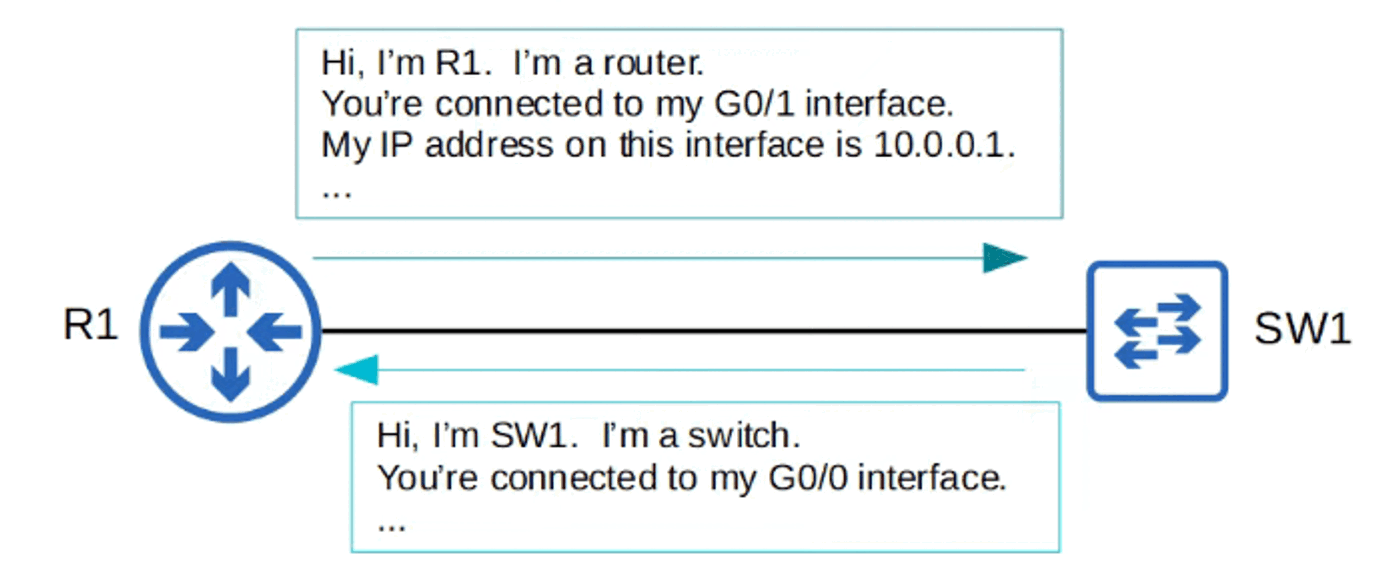
\includegraphics[keepaspectratio,alt={image}]{images/37-cdp-and-lldp/img-001.png}}
\end{figure}

\section{Cisco Discovery Protocol
(CDP)}\label{cisco-discovery-protocol-cdp}

\begin{itemize}
\tightlist
\item
  CDP is a Cisco proprietary protocol
\item
  It is enabled on Cisco devices (routers, switches, firewalls, IP
  Phones, etc) by DEFAULT
\end{itemize}

\begin{tipbox}

CDP Messages are periodically sent to Multicast MAC ADDRESS
\passthrough{\lstinline!0100.0CCC.CCCC!}

\end{tipbox}

\begin{itemize}
\tightlist
\item
  When a DEVICE receives a CDP message, it PROCESSES and DISCARDS the
  message. It does NOT forward it to other devices.
\item
  By DEFAULT, CDP Messages are sent once every \textbf{60 seconds}
\item
  By DEFAULT, the CDP hold-time is \textbf{180 seconds.} If a message
  isn't received from a neighbor for 180 seconds, the neighbor is
  REMOVED from the CDP Neighbor Table
\item
  CDPv2 messages are sent by DEFAULT
\end{itemize}

\begin{figure}
\centering
\pandocbounded{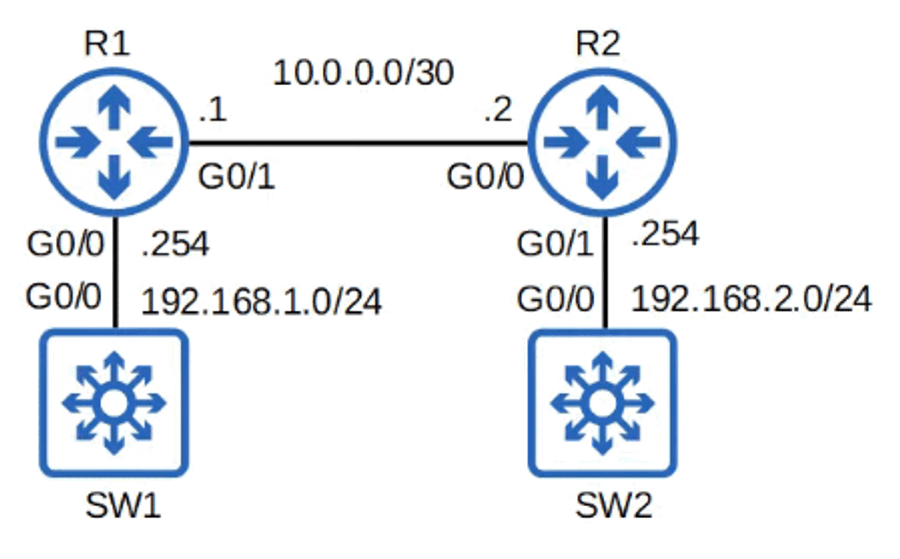
\includegraphics[keepaspectratio,alt={image}]{images/37-cdp-and-lldp/img-002.png}}
\end{figure}

\begin{figure}
\centering
\pandocbounded{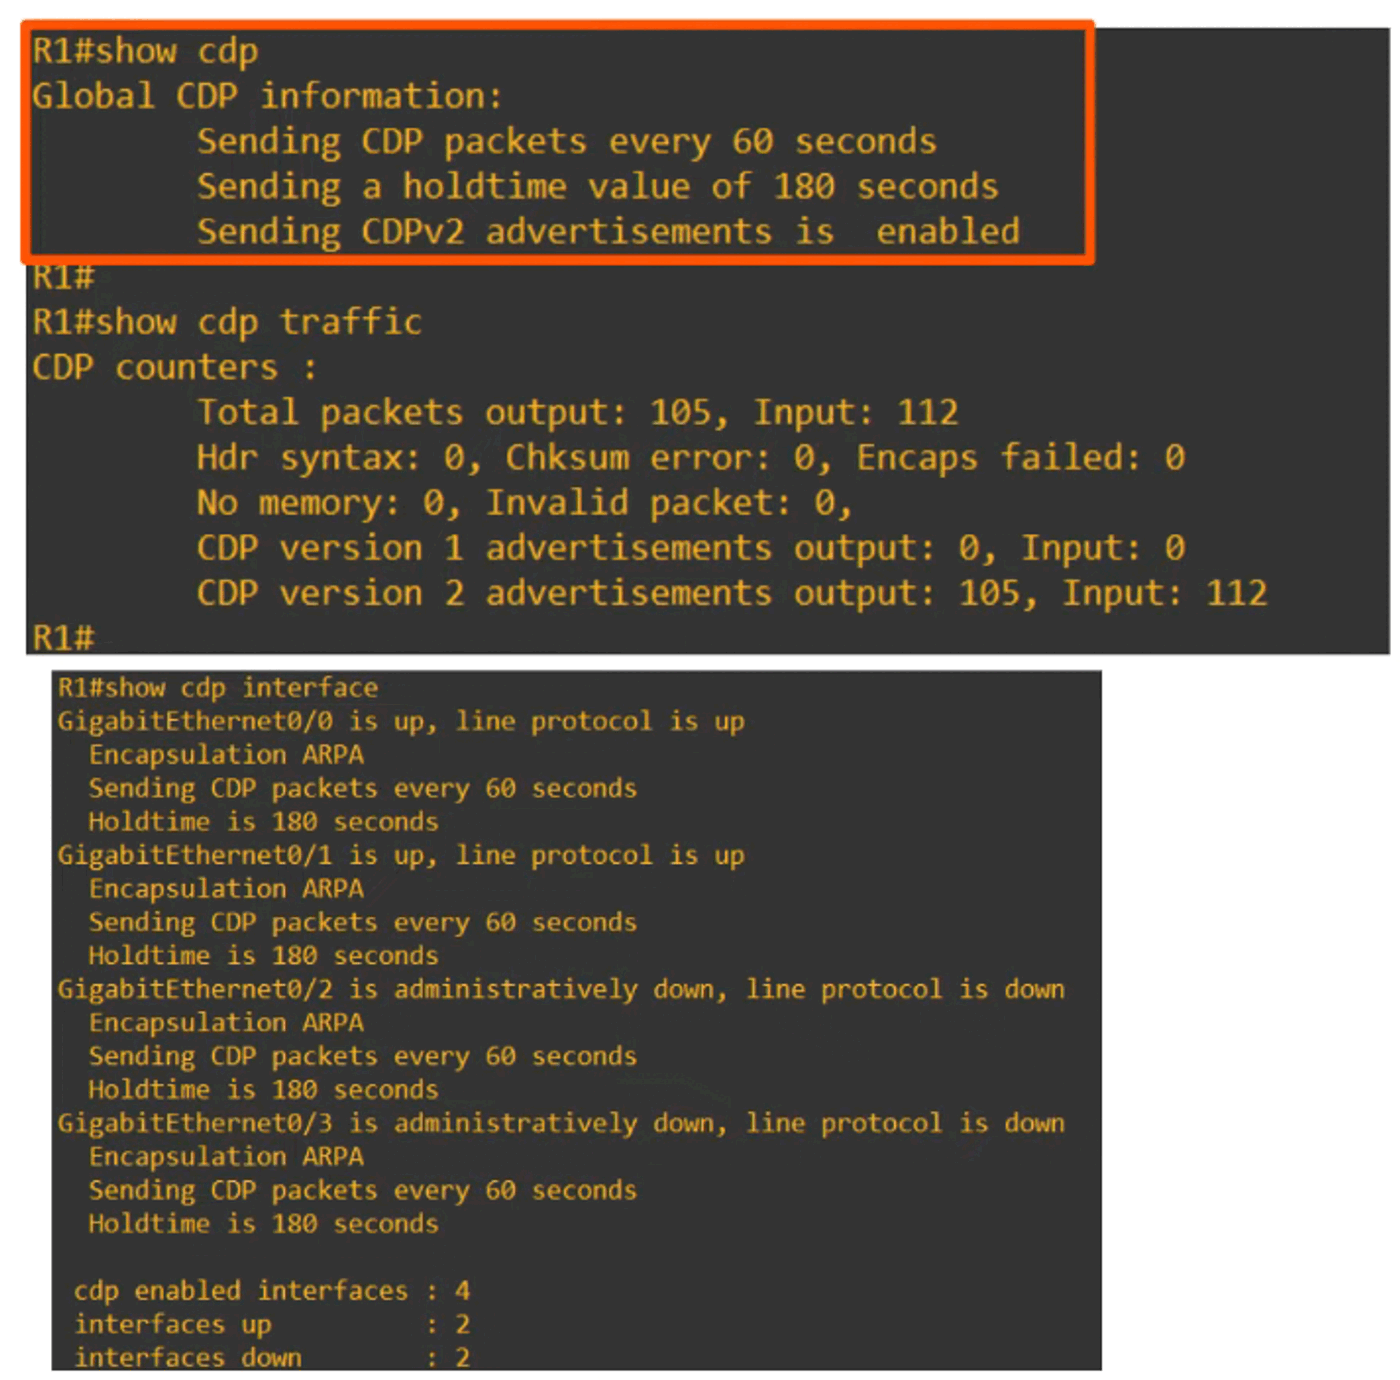
\includegraphics[keepaspectratio,alt={image}]{images/37-cdp-and-lldp/img-003.png}}
\end{figure}

\section{CDP Neighbor Tables}\label{cdp-neighbor-tables}

\begin{figure}
\centering
\pandocbounded{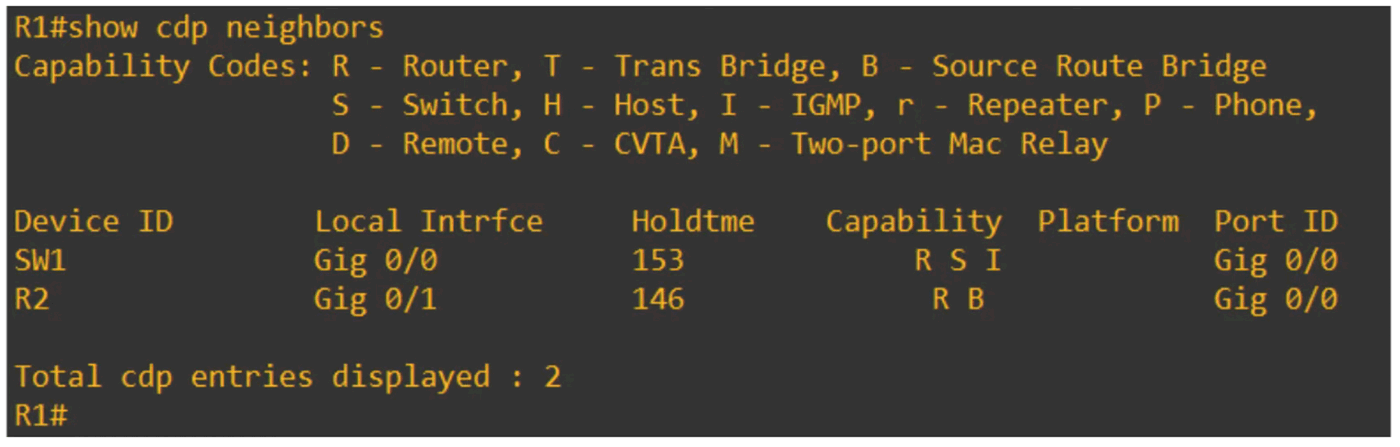
\includegraphics[keepaspectratio,alt={image}]{images/37-cdp-and-lldp/img-004.png}}
\end{figure}

``Device ID'' = What devices were DISCOVERED by CDP

``Local Intrface'' = What LOCAL device interface the neighbors are
connected to

``Holdtime'' = Hold-time countdown in seconds (0 = device removed from
table)

``Capabilities'' = Refers to Capability Codes table (located above
output)

``Platform'' = Displays the MODEL of the Neighbor Device

``Port ID'' = Neighbor ports that LOCAL device is connected to

\section{More Detailed Output}\label{more-detailed-output}

\begin{figure}
\centering
\pandocbounded{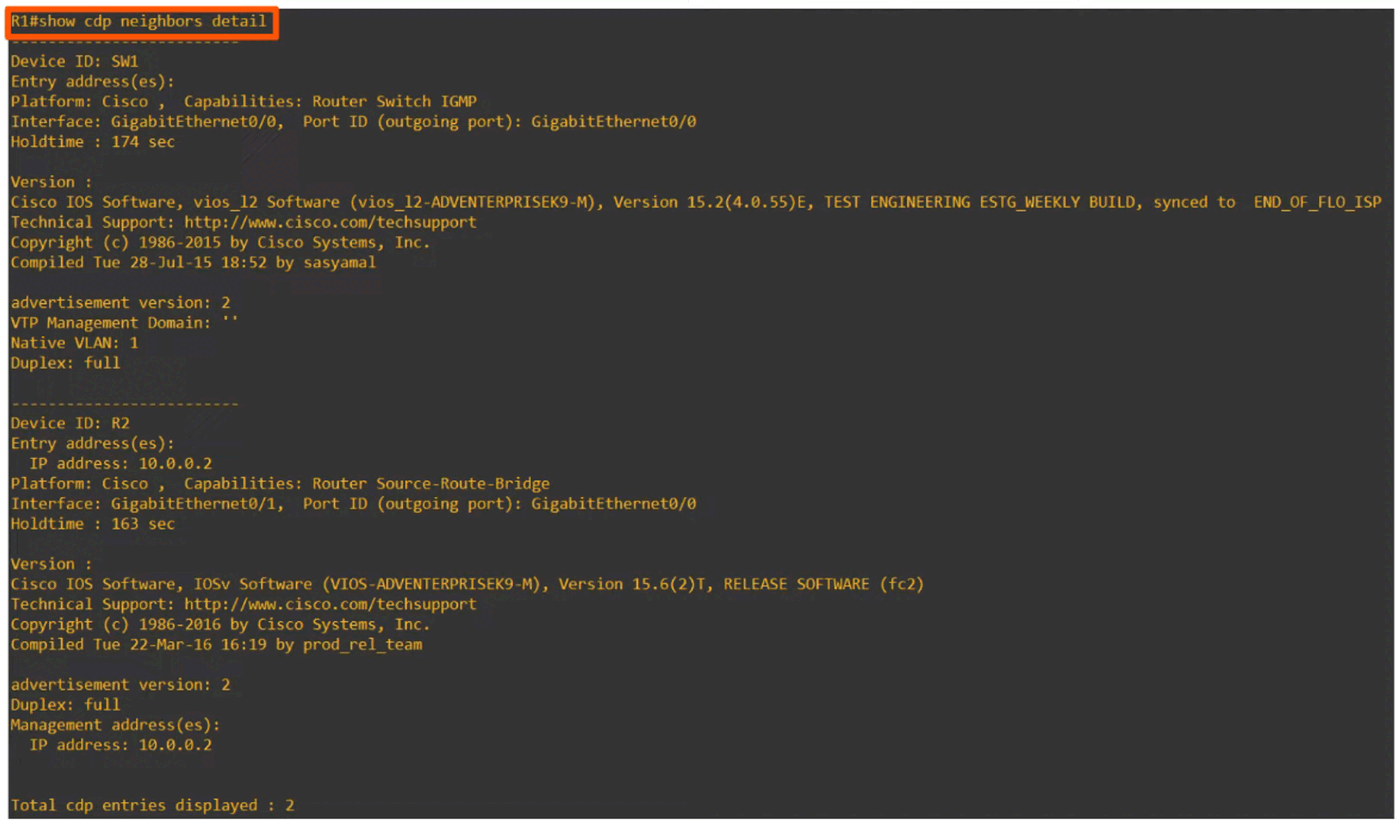
\includegraphics[keepaspectratio,alt={image}]{images/37-cdp-and-lldp/img-005.png}}
\end{figure}

``Version'' = shows what version of Cisco's IOS is running on the device

\section{Show Specific CDP Neighbor
Entry}\label{show-specific-cdp-neighbor-entry}

\begin{figure}
\centering
\pandocbounded{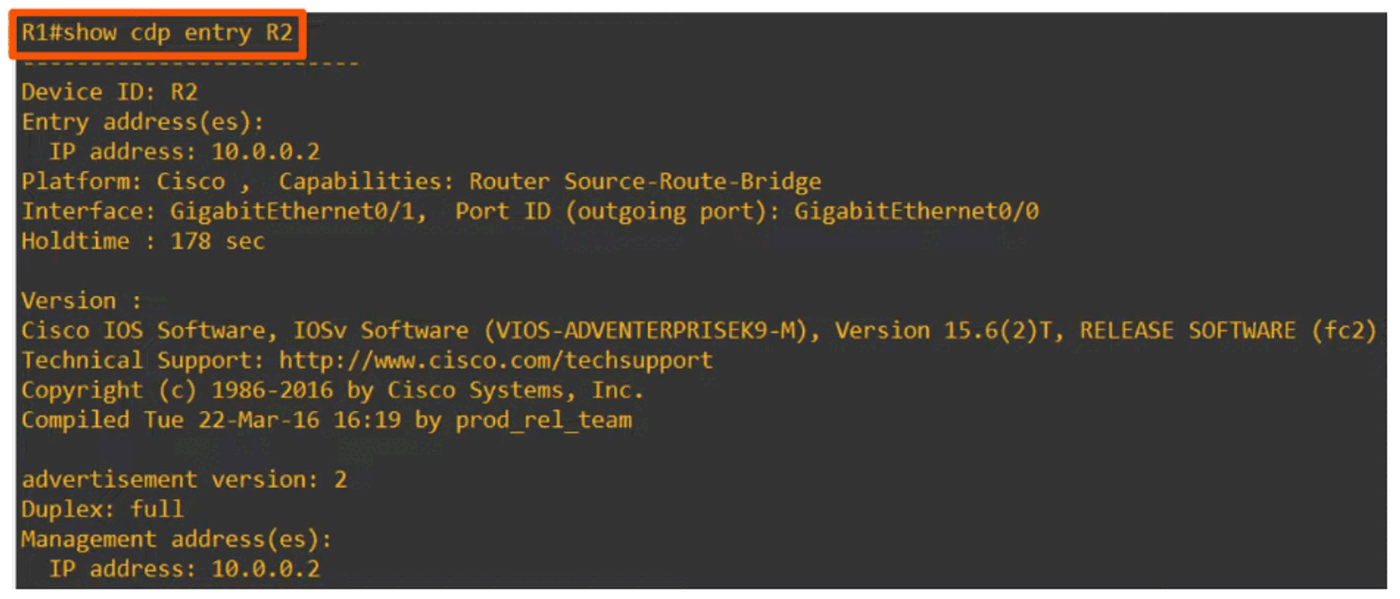
\includegraphics[keepaspectratio,alt={image}]{images/37-cdp-and-lldp/img-006.png}}
\end{figure}

\section{CDP Configuration Commands}\label{cdp-configuration-commands}

\begin{figure}
\centering
\pandocbounded{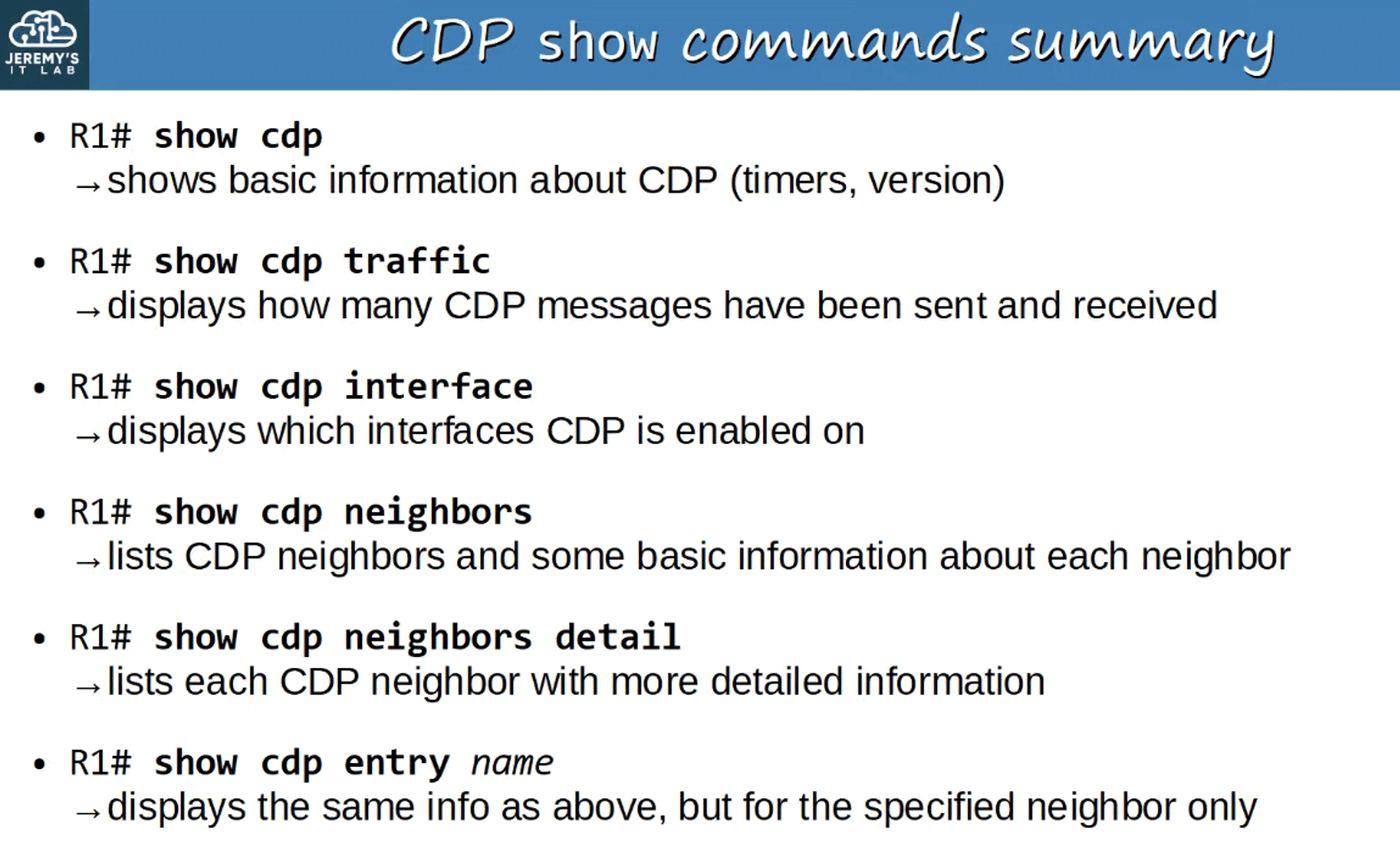
\includegraphics[keepaspectratio,alt={image}]{images/37-cdp-and-lldp/img-007.png}}
\end{figure}

\begin{itemize}
\tightlist
\item
  CDP is GLOBALLY ENABLED, by DEFAULT
\item
  CDP is also ENABLED on each INTERFACE, by DEFAULT
\item
  To ENABLE / DISABLE CDP globally:
  \passthrough{\lstinline!R1(config)\# [no] cdp run!}
\item
  To ENABLE / DISABLE CDP on specific interfaces :
  \passthrough{\lstinline!R1(config-if)\# [no] cdp enable!}
\item
  Configure the CDP timer:
  \passthrough{\lstinline!R1(config)\# cdp time *seconds*!}
\item
  Configure the CDP holdtime:
  \passthrough{\lstinline!R1(config)\# cdp holdtime *seconds*!}
\item
  ENABLE / DISABLE CDPv2:
  \passthrough{\lstinline!R1(config)\# [no] cdp advertise-v2!}
\end{itemize}

\section{Link Layer Discovery Protocol
(LLDP)}\label{link-layer-discovery-protocol-lldp}

\begin{itemize}
\tightlist
\item
  LLDP is an INDUSTRY STANDARD PROTOCOL (IEEE 802.1AB)
\item
  It is usually DISABLED on Cisco devices, by DEFAULT, so it must be
  manually ENABLED
\item
  A device can run CDP and LLDP at the same time
\end{itemize}

\begin{tipbox}

LLDP Messages are periodically sent to Multicast MAC ADDRESS
\passthrough{\lstinline!0180.c200.000E!}

\end{tipbox}

\begin{itemize}
\tightlist
\item
  When a DEVICE receives an LLDP message, it PROCESSES and DISCARDS the
  message. It does NOT forward it to OTHER DEVICES
\item
  By DEFAULT, LLDP Messages are sent once every \textbf{30 seconds}
\item
  By DEFAULT, LLDP Holdtime is \textbf{120 seconds}
\item
  LLDP has an additional timer called the `reinitialization delay'

  \begin{itemize}
  \tightlist
  \item
    If LLDP is ENABLED (Globally or on an INTERFACE), this TIMER will
    DELAY the actual initialization of LLDP (\textbf{2 seconds,} by
    DEFAULT)
  \end{itemize}
\end{itemize}

\section{LLDP Configuration Commands}\label{lldp-configuration-commands}

\begin{itemize}
\item
  LLDP is usually GLOBALLY DISABLED by DEFAULT
\item
  LLDP is also DISABLED on each INTERFACE, by DEFAULT
\item
  To ENABLE LLDP GLOBALLY :
  \passthrough{\lstinline!R1(config)\# lldp run!}
\item
  To ENABLE LLDP on specific INTERFACES (tx):
  \passthrough{\lstinline!R1(config-if)\# lldp transmit!}
\item
  To ENABLE LLDP on specific INTERFACES (rx):
  \passthrough{\lstinline!R1(config-if)\# lldp receive!}
\end{itemize}

YOU NEED TO ENABLE BOTH TO SEND AND RECEIVE (Unless you want to only
enable SEND or RECEIVE LLDP Messages)

\begin{itemize}
\tightlist
\item
  Configure the LLDP timer:
  \passthrough{\lstinline!R1(config)\# lldp timer *seconds*!}
\item
  Configure the LLDP holdtime:
  \passthrough{\lstinline!R1(config)\# lldp holdtime *seconds*!}
\item
  Configure the LLDP reinit timer:
  \passthrough{\lstinline!R1(config)\# lldp reinit *seconds*!}
\end{itemize}

\begin{figure}
\centering
\pandocbounded{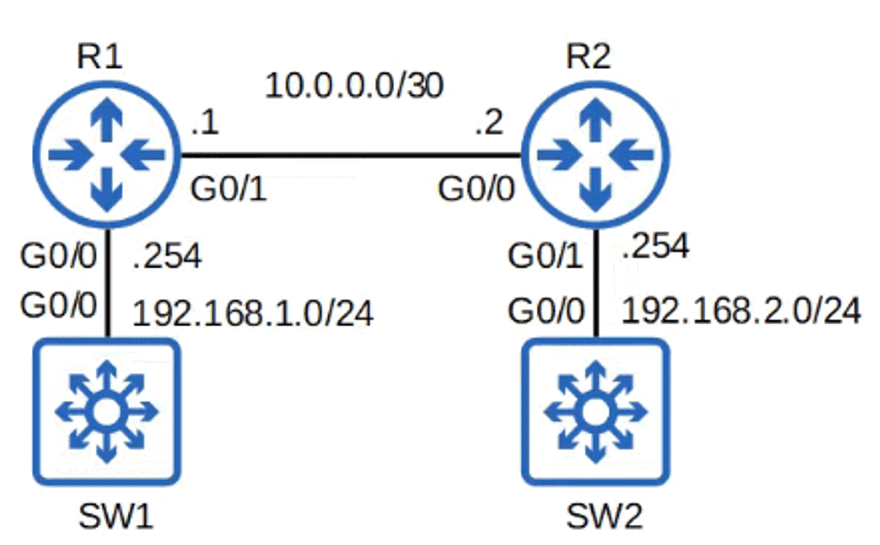
\includegraphics[keepaspectratio,alt={image}]{images/37-cdp-and-lldp/img-008.png}}
\end{figure}

\begin{figure}
\centering
\pandocbounded{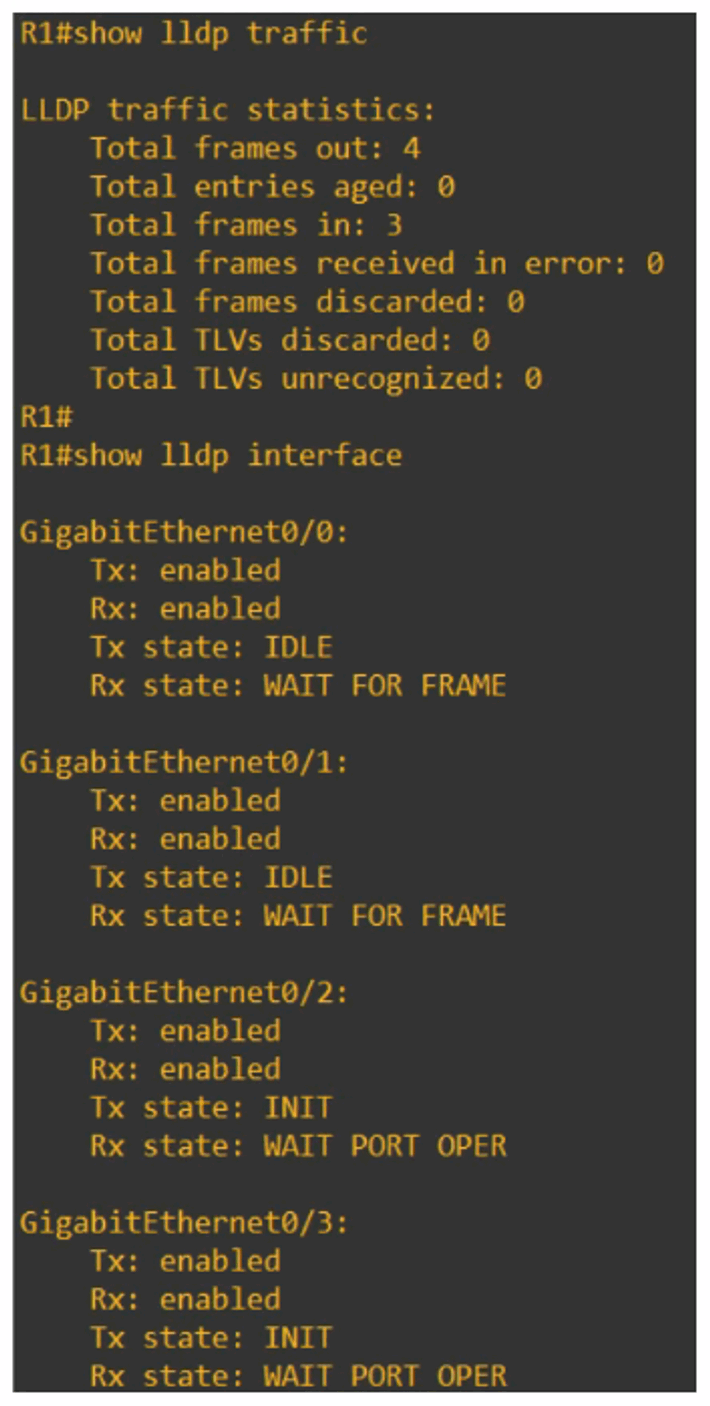
\includegraphics[keepaspectratio,alt={image}]{images/37-cdp-and-lldp/img-009.png}}
\end{figure}

\section{Show LLDP Status}\label{show-lldp-status}

\begin{figure}
\centering
\pandocbounded{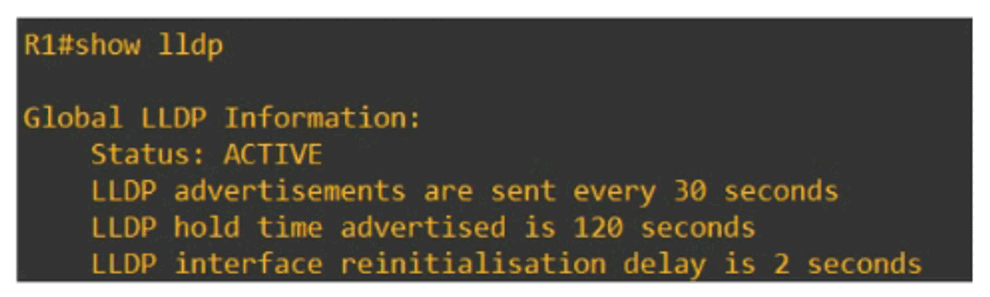
\includegraphics[keepaspectratio,alt={image}]{images/37-cdp-and-lldp/img-010.png}}
\end{figure}

\section{Show All LLDP Neighbors}\label{show-all-lldp-neighbors}

\begin{figure}
\centering
\pandocbounded{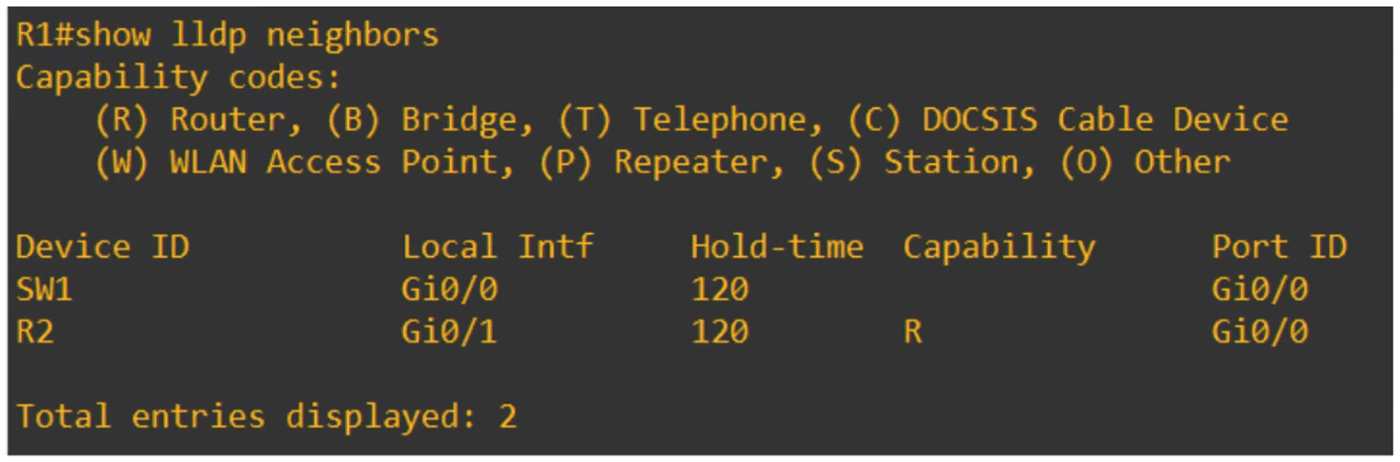
\includegraphics[keepaspectratio,alt={image}]{images/37-cdp-and-lldp/img-011.png}}
\end{figure}

SHOW LLDP NEIGHBORS in DETAIL

\begin{figure}
\centering
\pandocbounded{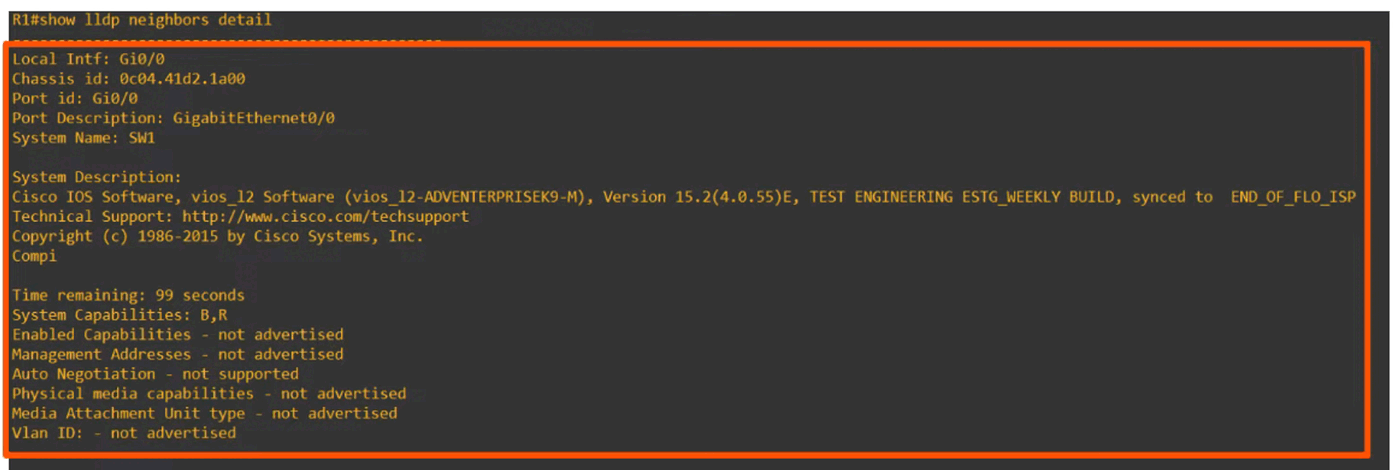
\includegraphics[keepaspectratio,alt={image}]{images/37-cdp-and-lldp/img-012.png}}
\end{figure}

\section{Show Specific LLDP Device
Entry}\label{show-specific-lldp-device-entry}

\begin{figure}
\centering
\pandocbounded{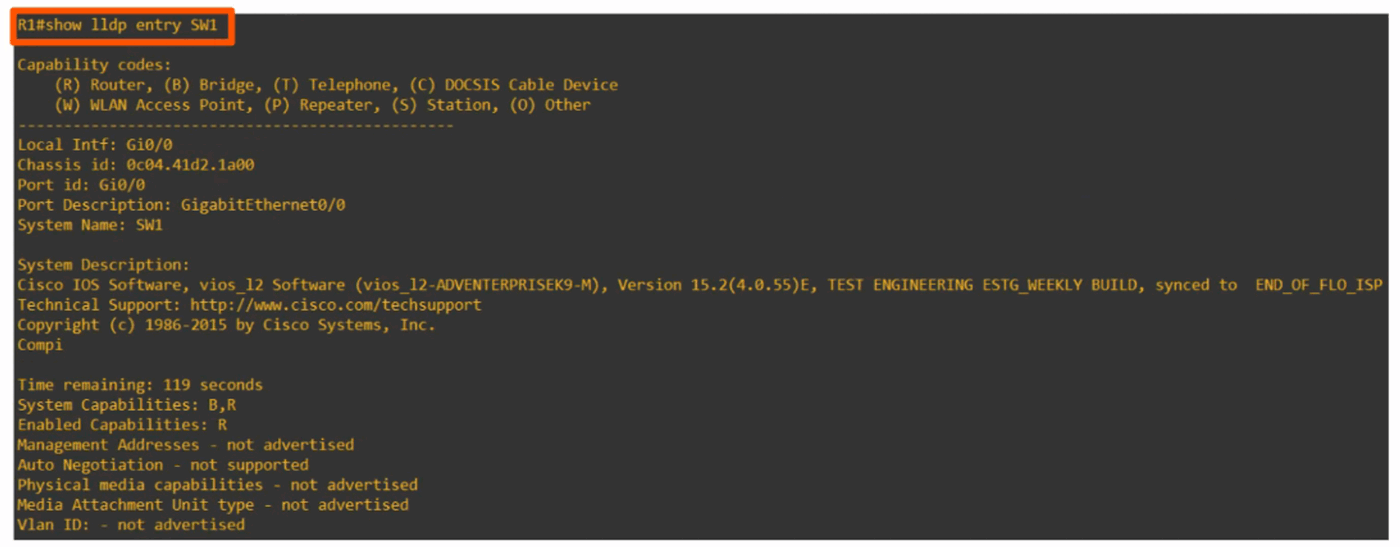
\includegraphics[keepaspectratio,alt={image}]{images/37-cdp-and-lldp/img-013.png}}
\end{figure}

\begin{figure}
\centering
\pandocbounded{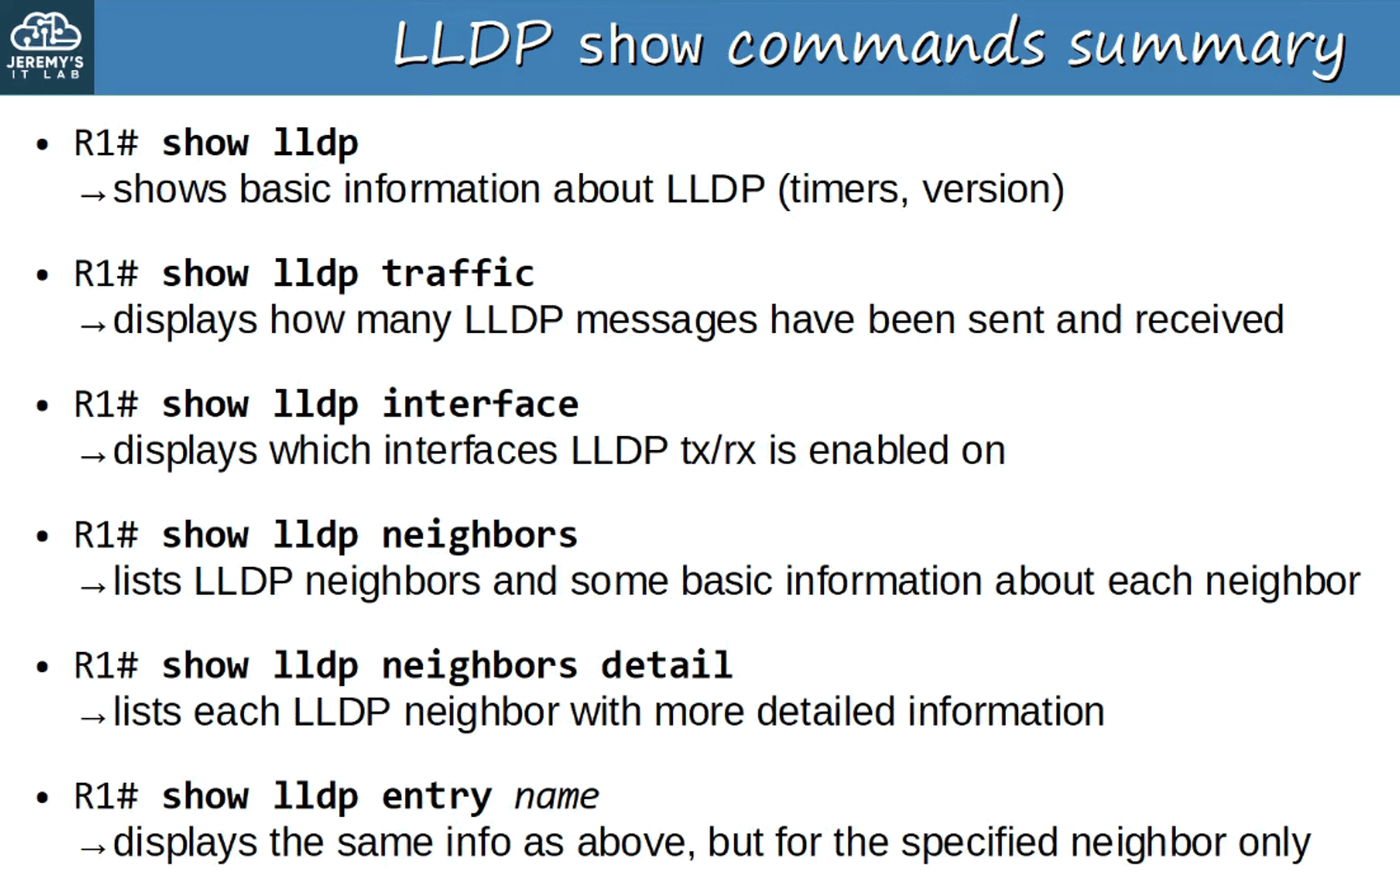
\includegraphics[keepaspectratio,alt={image}]{images/37-cdp-and-lldp/img-014.png}}
\end{figure}
